% \chapter{Модели пограничного слоя атмосферы}
\chapter{Пограничный слой атмосферы и его модели}

    % Весь этот раздел согласовать с лекциями ВМС 
    % см. https://www.notion.so/2a3f260c6bd3478b9014e1eceb9f3bbf


    \begin{figure}[h]
         \centering
         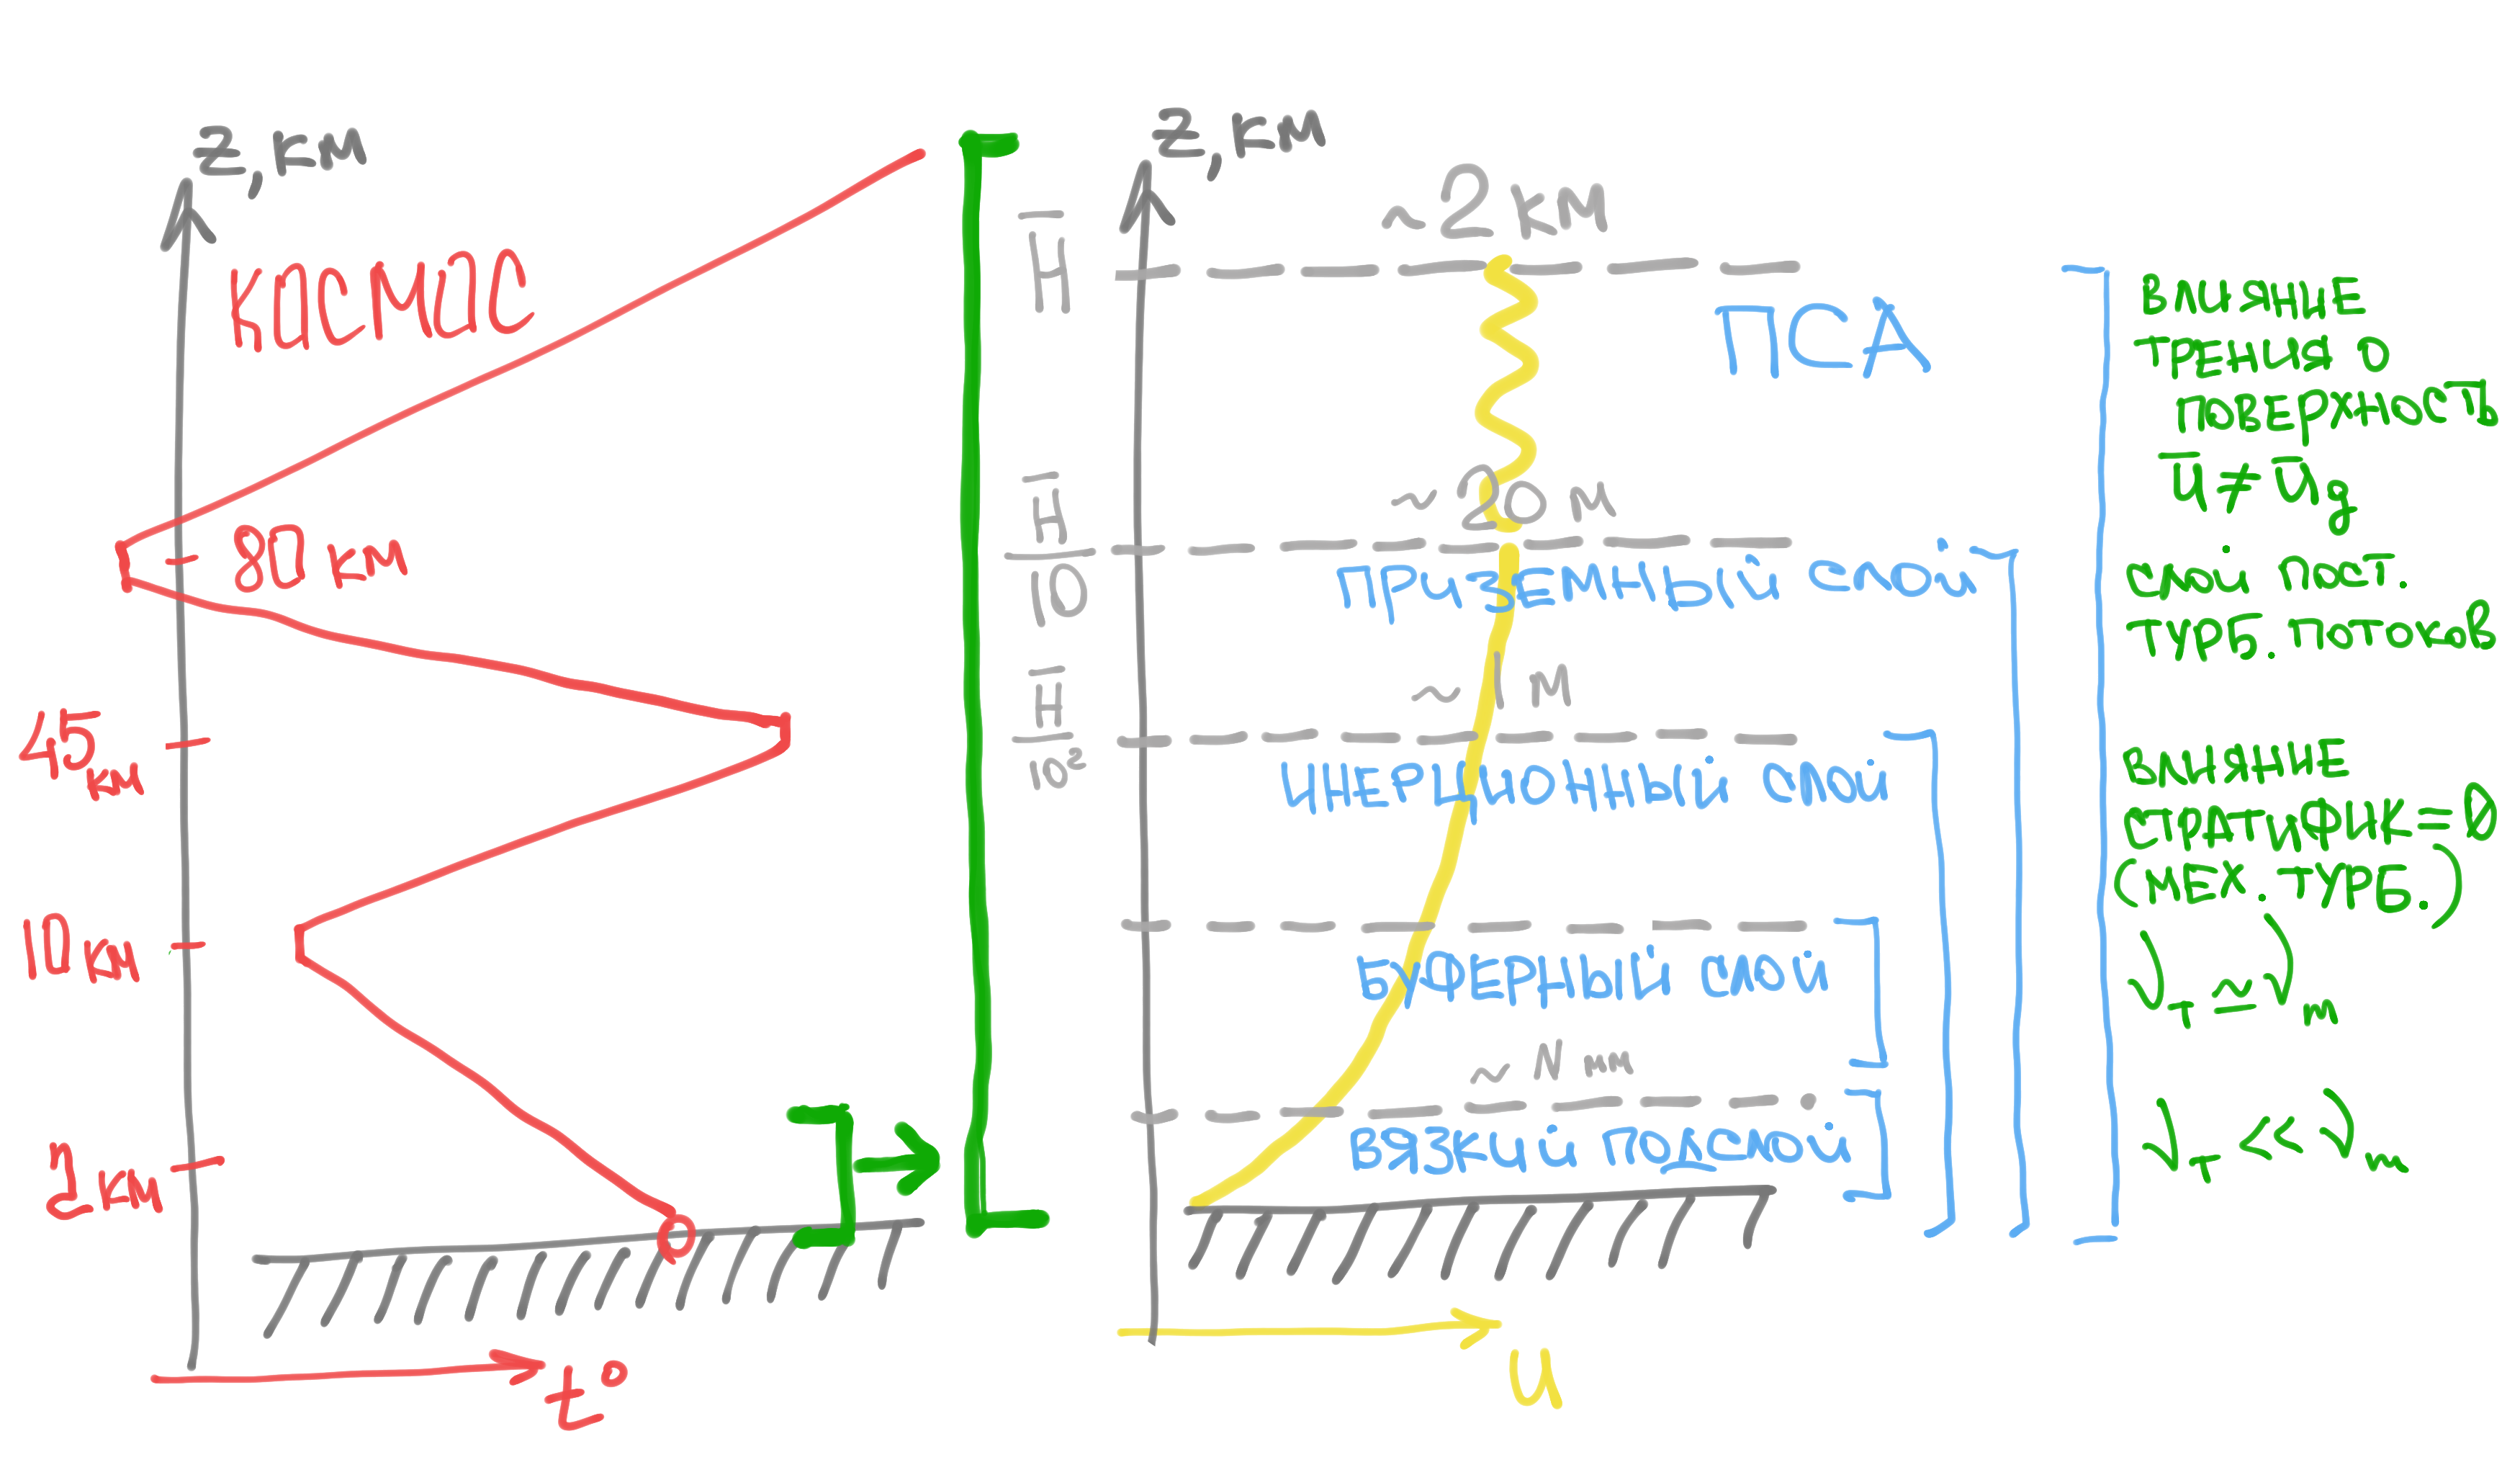
\includegraphics[width=1\linewidth]{pics/ch14_Atmos.png}
    \caption{\label{fig:ch14_Atmos} {\color{red}Строение атмосферы и ПСА. Схема из лекции. Можно как-то здесь применить? }}
    \end{figure}



Из самого определения следует, что пограничными должны называть слои, расположенные вблизи границ. Границы могут быть внешними, когда жидкость ограничивается каким-либо телом. Для атмосферы таким телом является поверхность Земли т.е. поверхность суши или океана. Могут быть также и внутренние пограничные слои, в которых резко изменяются какие-либо свойства жидкости. В атмосфере таким довольно устойчивым внутренним слоем является слой в окрестности тропопаузы. 

\begin{warn}
    Вставить про разные слои внутри ПСА \\
    (лекция ВМС https://youtu.be/KFWEeFD8dPM) \\
    расписать их размеры по широте.
\end{warn}

Ниже будет рассмотрен только внешний слой пограничный слой вблизи поверхности Земли, поэтому в дальнейшем прилагательное <<внешний>> использоваться не будет. 

\textbf{Пограничным слоем атмосферы} называется нижний 1--2 километровый (в среднем) слой атмосферы, в пределах которого распределение метеорологических величин определяется непосредственно влиянием подстилающей поверхности и турбулентностью. С точки зрения динамического взаимодействия атмосферы с подстилающей поверхностью существенным является то, что в случае суши, скорость ветра у поверхности равна нулю, т.е. поверхность оказывает тормозящее влияние на воздушные потоки. При этом неизбежно возникают поверхностные напряжения, который вызывают микромасштабную неустойчивость. Эту неустойчивость обобщенно можно называть турбулентностью, понимая под ней вихри небольшого масштаба. Возникновение таких вихрей обеспечивает обмен количеством движения, теплом и влагой между границей и внутренними слоями жидкости и некоторое сглаживание скорости. В случае идеального скольжения жидкости вдоль поверхности мы бы имели разрыв производной на границе (рис. \ref{fig:ch14_bl} (а)). Вязкость и турбулентность не допускает этого: они обеспечивают более гладкое приближение потока к границе (рис. \ref{fig:ch14_bl} (б)), но тем не менее сохраняется область повышенных значений градиента скорости, которая называется динамическим пограничным слоем. 
    \begin{figure}
    \begin{minipage}[b]{.52\textwidth} % left
        \centering
        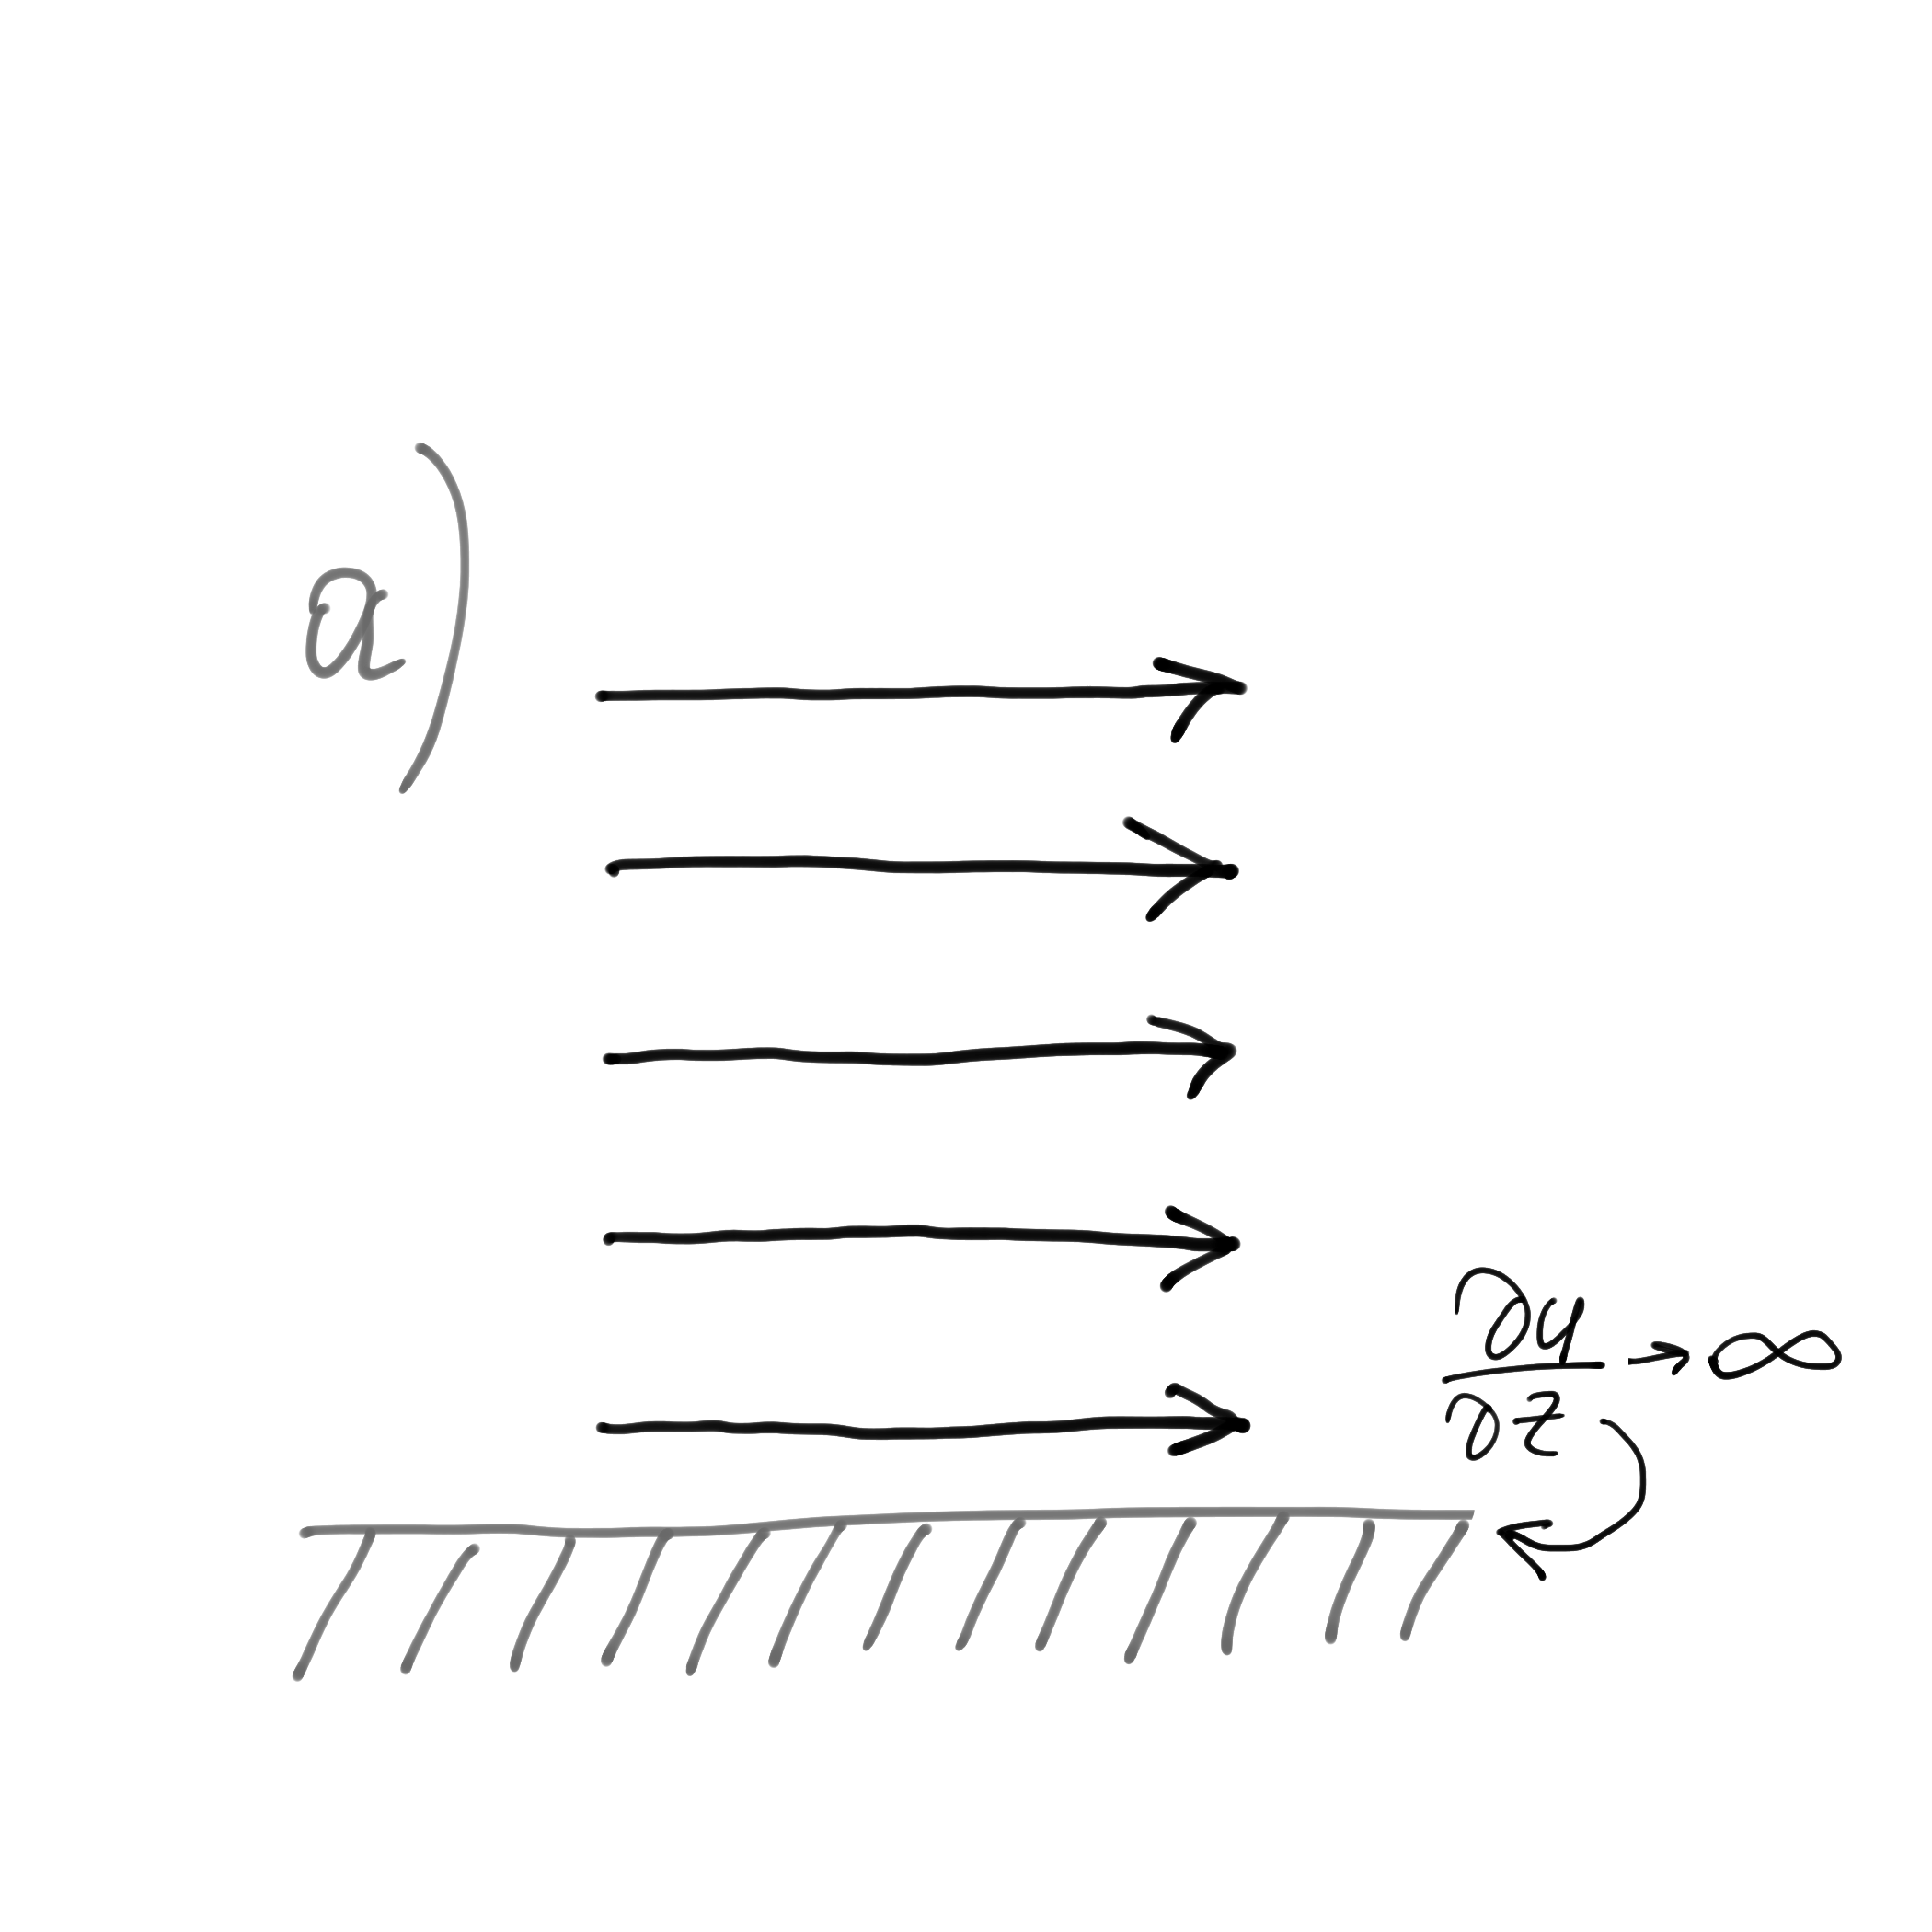
\includegraphics[width=1\linewidth]{pics/ch14_bl_a.png}
        \end{minipage}%
    \begin{minipage}[b]{.48\textwidth} % right
      \centering
      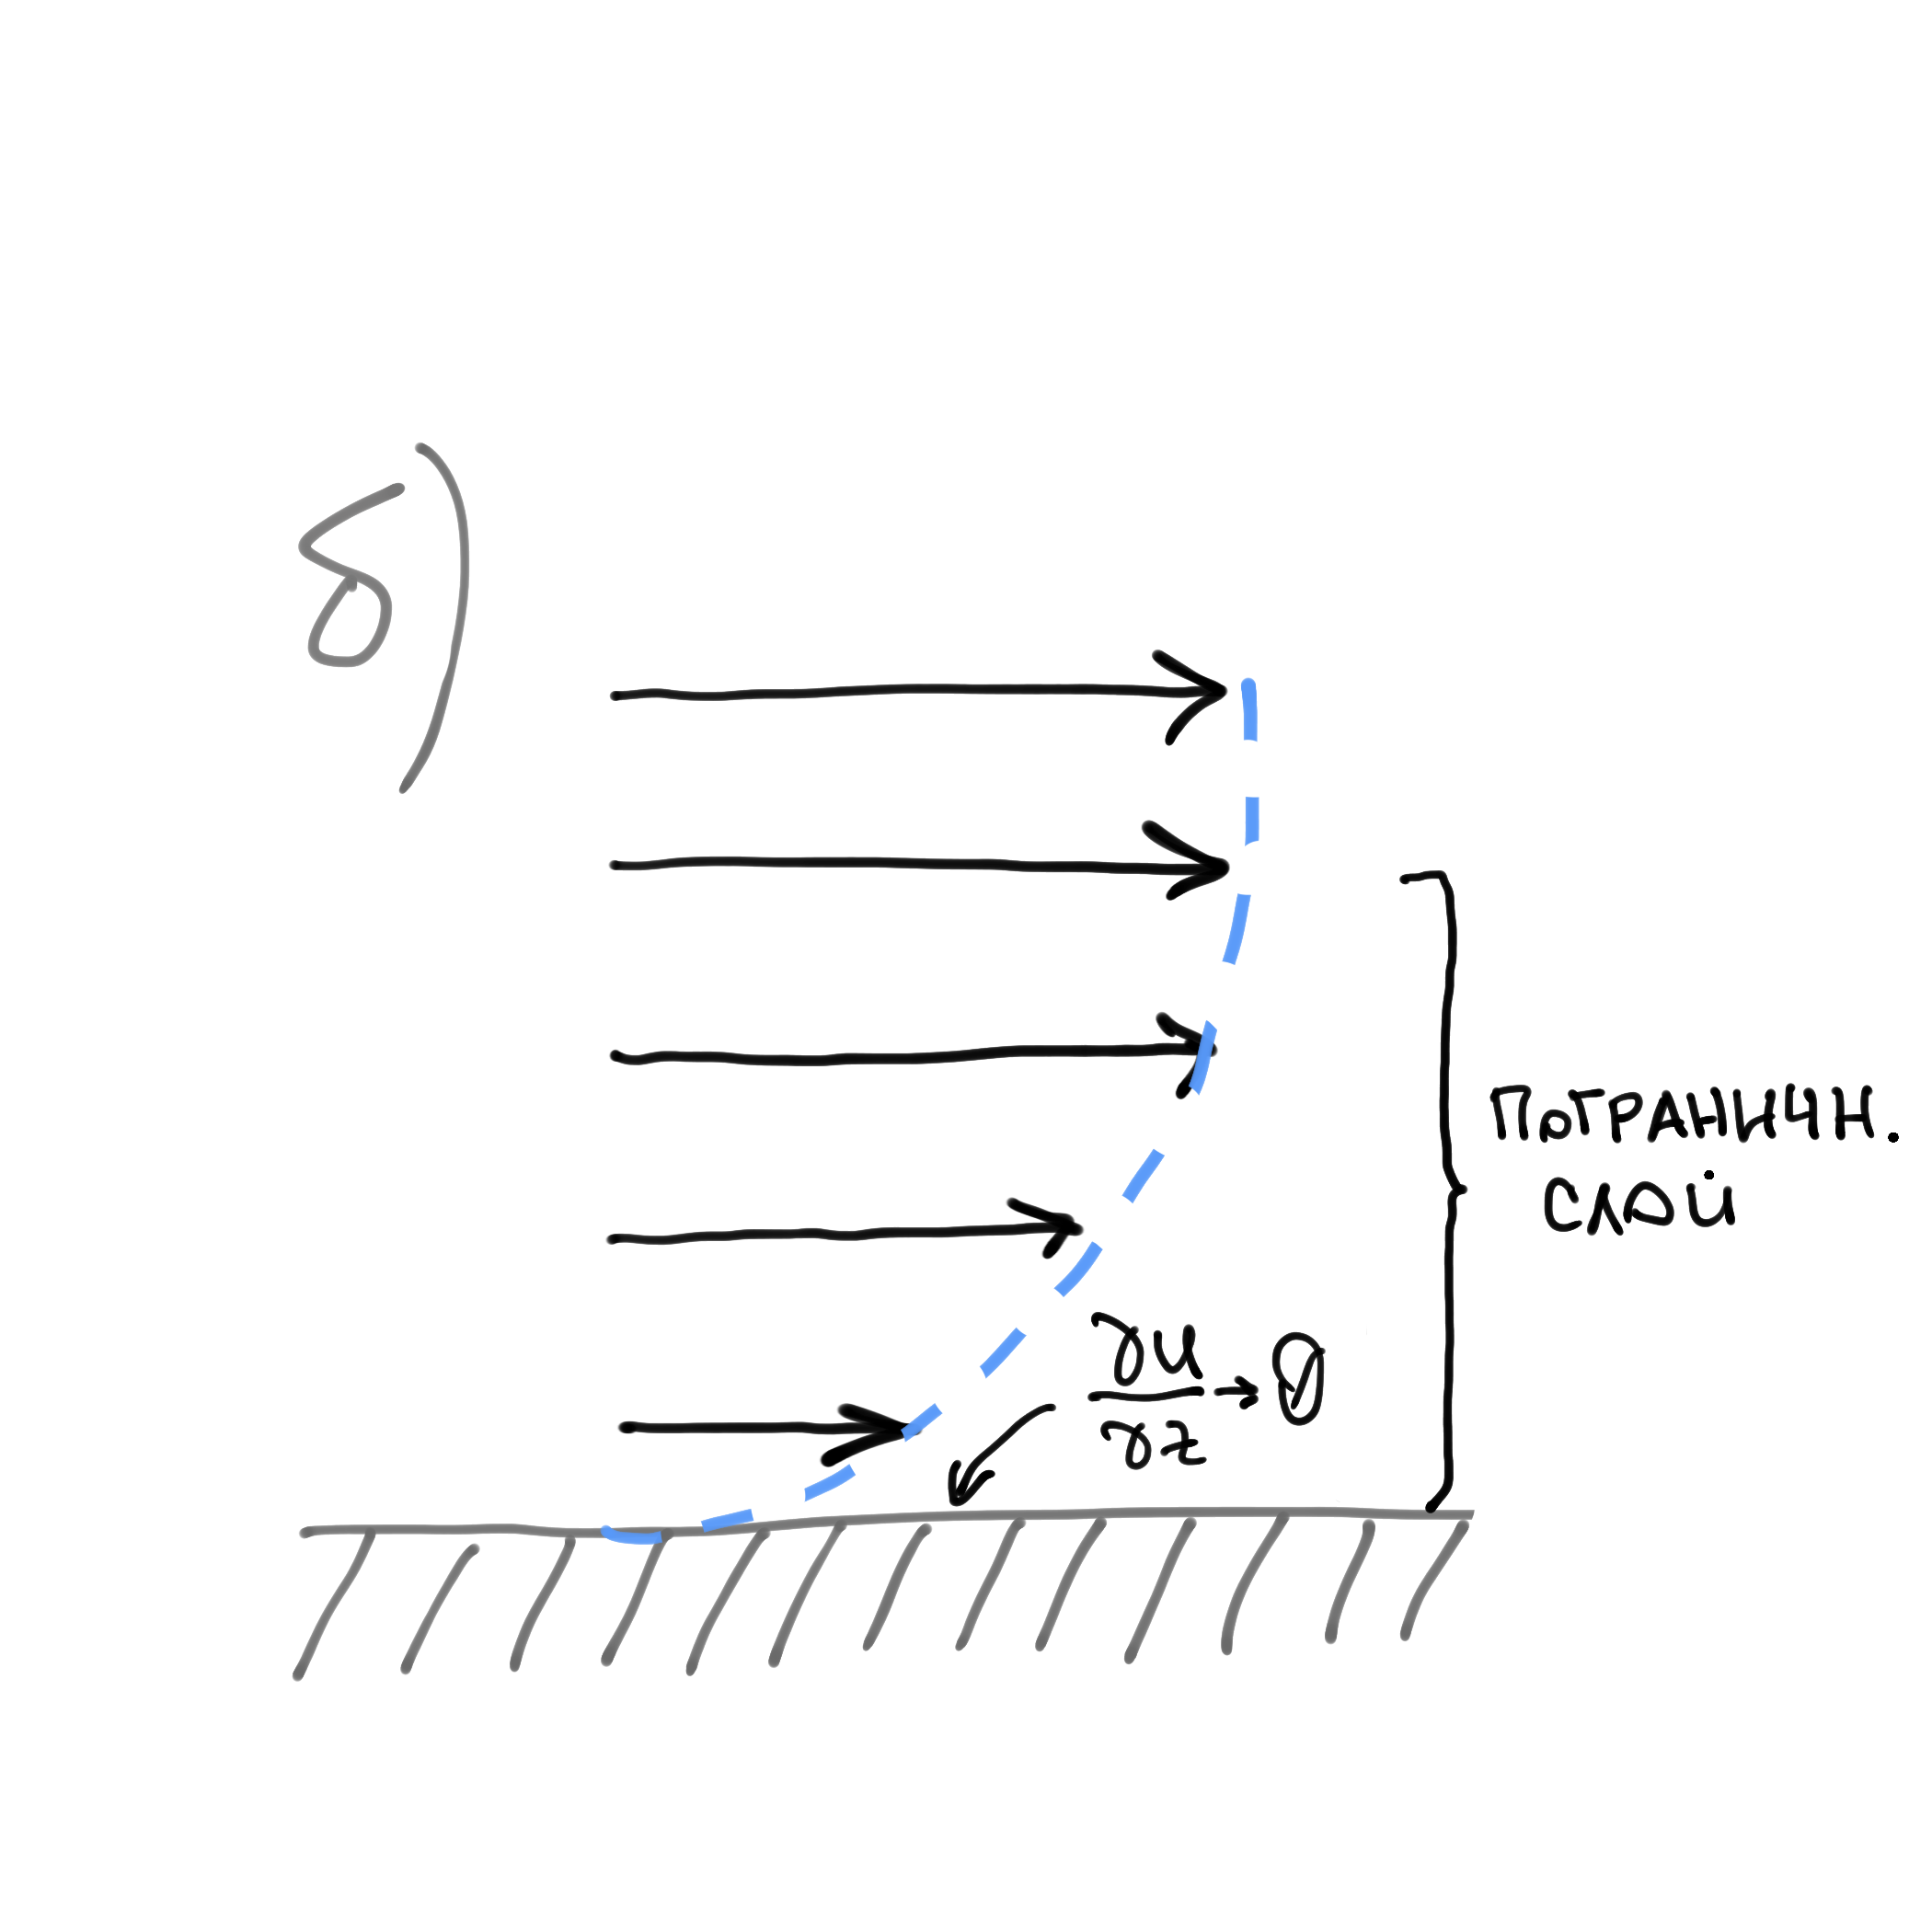
\includegraphics[width=1\linewidth]{pics/ch14_bl_b.png}
    \end{minipage}
    \caption{\label{fig:ch14_bl} {\color{red}Схема скольжения воздуха о поверхность в случае идеальной  (а) и вязкой (б) жидкости }}
    \end{figure}

Для поверхности Земли характерны также наибольшие притоки солнечной радиации и стоки тепла вследствие излучения в ИК-области спектра, гораздо больше, чем это имеет место в слое атмосферы, прилегающем к поверхности Земли, поэтому здесь имеет место и термический пограничный слой. Мы не будем в дальнейшем подразделять два этих фактора: термический и динамический, а будем рассматривать эту проблему с общей позиции теории подобия.

\section{{\color{done}Простая стационарная модель пограничного слоя}}

В более простых задачах пограничного слоя, которые будут рассматриваться ниже, применяется ряд упрощающих гипотез:
\begin{itemize}
  \item процесс считается стационарным $\td{}{t}=0$,
  \item принимается однородность потока в горизонтальном направлении, т.е. $\pd{}{x}=\pd{}{y}=0$,
  \item движения считываются плоскими.
\end{itemize}

В этом случае уравнения движения приобретает вид

\begin{align}
    \pd{}{z}k\pd{u}{z}+fv=\frac{1}{\rho}\pd{p}{x}, \label{eq:ch14_1} \\
    \pd{}{z}k\pd{v}{z}-fu=\frac{1}{\rho}\pd{p}{y}. \label{eq:ch14_2} 
\end{align}
Если считать градиент давления внешним параметром, т.е. параметром, определяемым из каких-то других соотношений, не связанных с уравнениями (\ref{eq:ch14_1})-(\ref{eq:ch14_2}), например из условий гидростатичности потока
\begin{equation*}
    v_g=\frac{1}{\rho f}\pd{p}{x}, \:\:\: u_g=-\frac{1}{\rho f}\pd{p}{y},
\end{equation*}
то уравнения (\ref{eq:ch14_1})-(\ref{eq:ch14_2}) можно представить в виде
\begin{align}
    \pd{}{z}k\pd{u}{z}+f(v-v_g)=0 \label{eq:ch14_3}, \\
    \pd{}{z}k\pd{v}{z}-f(u-u_g)=0 \label{eq:ch14_4}.
\end{align}
Эти уравнения часто используются в качестве исходных при изучении пограничного слоя.

Внутри атмосферного пограничного слоя выделяют также \textit{приземный слой} толщиной порядка нескольких десятков метров, в котором эмпирически наблюдается постоянство потоков тепла, количества движения или субстанций (например влажности). 

Исходные уравнения, используемые при рассмотрении приземного слоя, имеют несколько иной вид. 

Так как в этом тонком слое не имеет значение ориентация воздушного потока, ориентируют обычно с каким-нибудь одним компонентом скорости, подразумевая под ним просто модуль вектора скорости. Пусть это будет $u$.

В разделе {\color{red}ссылка} уже выводились уравнения для осредненного потока, которые имели вид

 \begin{equation}
 \label{eq:ch14_5} 
     \td{\overline{u}}{t}=-\frac{1}{ \overline{p} }\pd{\overline{p}}{x} 
        -\pd{(\overline{u^{'}}^{2})}{x} 
        -\pd{(\overline{u^{'}v^{'}})}{y} 
        -\pd{ (\overline{u^{'}w^{'}})}{z}  
\end{equation}
\begin{equation*}
         ... 
\end{equation*}
 \begin{equation}
 \label{eq:ch14_6}
         \td{\overline{\theta}}{t}= 
        -\pd{(\overline{u^{'}\theta^{'}})}{x} 
        -\pd{(\overline{\theta^{'}v^{'}})}{y} 
        -\pd{ (\overline{\theta^{'}w^{'}})}{z}  
  \end{equation}
Если теперь мы введем гипотезу о стационарности и периодичности движений в горизонтальном направлении, пренебрежем силами градиента давления, но введем вязкость и температуропроводность, то уравнения (\ref{eq:ch14_5}) и (\ref{eq:ch14_6}) приобретут вид
\begin{align}
    0&=-\pd{(\overline{u^{'}w^{'}})}{z} + \nu \pd{^2 u}{z^2}, \label{eq:ch14_7} \\
    0&=-\pd{ (\overline{\theta^{'}w^{'}})}{z} + \varkappa \pd{^2 \theta}{z^2}.  \label{eq:ch14_8}
\end{align}
Вспоминаем, что градиенты представляет собой вектор, направленный в сторону роста функции, а поток направлен в сторону, обратную градиенту. Поэтому переходя от притоков (дивергенции потоков) к самим потокам, будем иметь из (\ref{eq:ch14_7})  и (\ref{eq:ch14_8}) (домножив \ref{eq:ch14_7} на $\rho$, а (\ref{eq:ch14_8}) на $\rho C_P$ для получения размерности потока импульса и тепла)
\begin{align}
    \tau &= \rho \overline{u^{'}w^{'}} - \rho \nu \pd{u}{z} = const, \label{eq:ch14_9} \\
    H &= C_P \rho \overline{w^{'} \theta^{'}} - \rho C_P \varkappa \pd{\theta}{z} = const. \label{eq:ch14_10}
\end{align}
Здесь $\tau$ -- вертикальный поток импульса, $H$ -- вертикальный поток тепла. Уравнения (\ref{eq:ch14_9}) и (\ref{eq:ch14_10}) будут являться для нас исходными при рассмотрении распределения метеорологических величин в приземном слое на основе теории подобия. Заметим дополнительно, что в уравнении притока тепла (\ref{eq:ch14_6}) и последующих уравнениях мы исключили из рассмотрения радиационные притоки (потоки) тепла, а также притоки (потоки) тепла за счет фазовых переходов влаги, считая их несущественными при наличии развитой турбулентности. В уравнении движения была отброшена сила Кориолиса из-за малости масштаба движения. 

В этом разделе мы рассмотрим последовательно две задачи: сначала задачу об изменении ветра с высотой в пограничном слое атмосферы (более крупномасштабную задачу, где учитывается сила Кориолиса), а затем задачу о распределении по вертикали метеорологических величин с использовании следствий из теории подобия, развитой применительно к атмосферному приземному слою в работах {\color{red}Монина и Обухова (1953, 1954). }

\section{{\color{done}Изменение ветра с высотой в планетарном пограничном слое}}
В однородной воздушной массе отчетливо проявляется увеличение скорости ветра с высотой, правое его вращение с северном полушарии и левое -- в южном. Такое изменение скорости с высотой начинается с высоты 10-20 м и распространяется в умеренных широтах до высоты около 1 км. Изменения направления ветра в пограничном слое обусловлено, очевидно, совместным действием отклоняющей силы вращения Земли и турбулентности. 

Слой в котором наблюдается вращение ветра с высотой, обусловленное действием турбулентности и отклоняющей силой вращения Земли, называется \textit{планетарным пограничным слоем}. Наиболее существенной характеристикой это слоя является угол $\Theta$, образуемый направлением ветра и изобарами, который часто называют <<углом поворота>> (рис. \ref{fig:ch14-2_wind_turn})
    \begin{figure}[h]
        \centering
        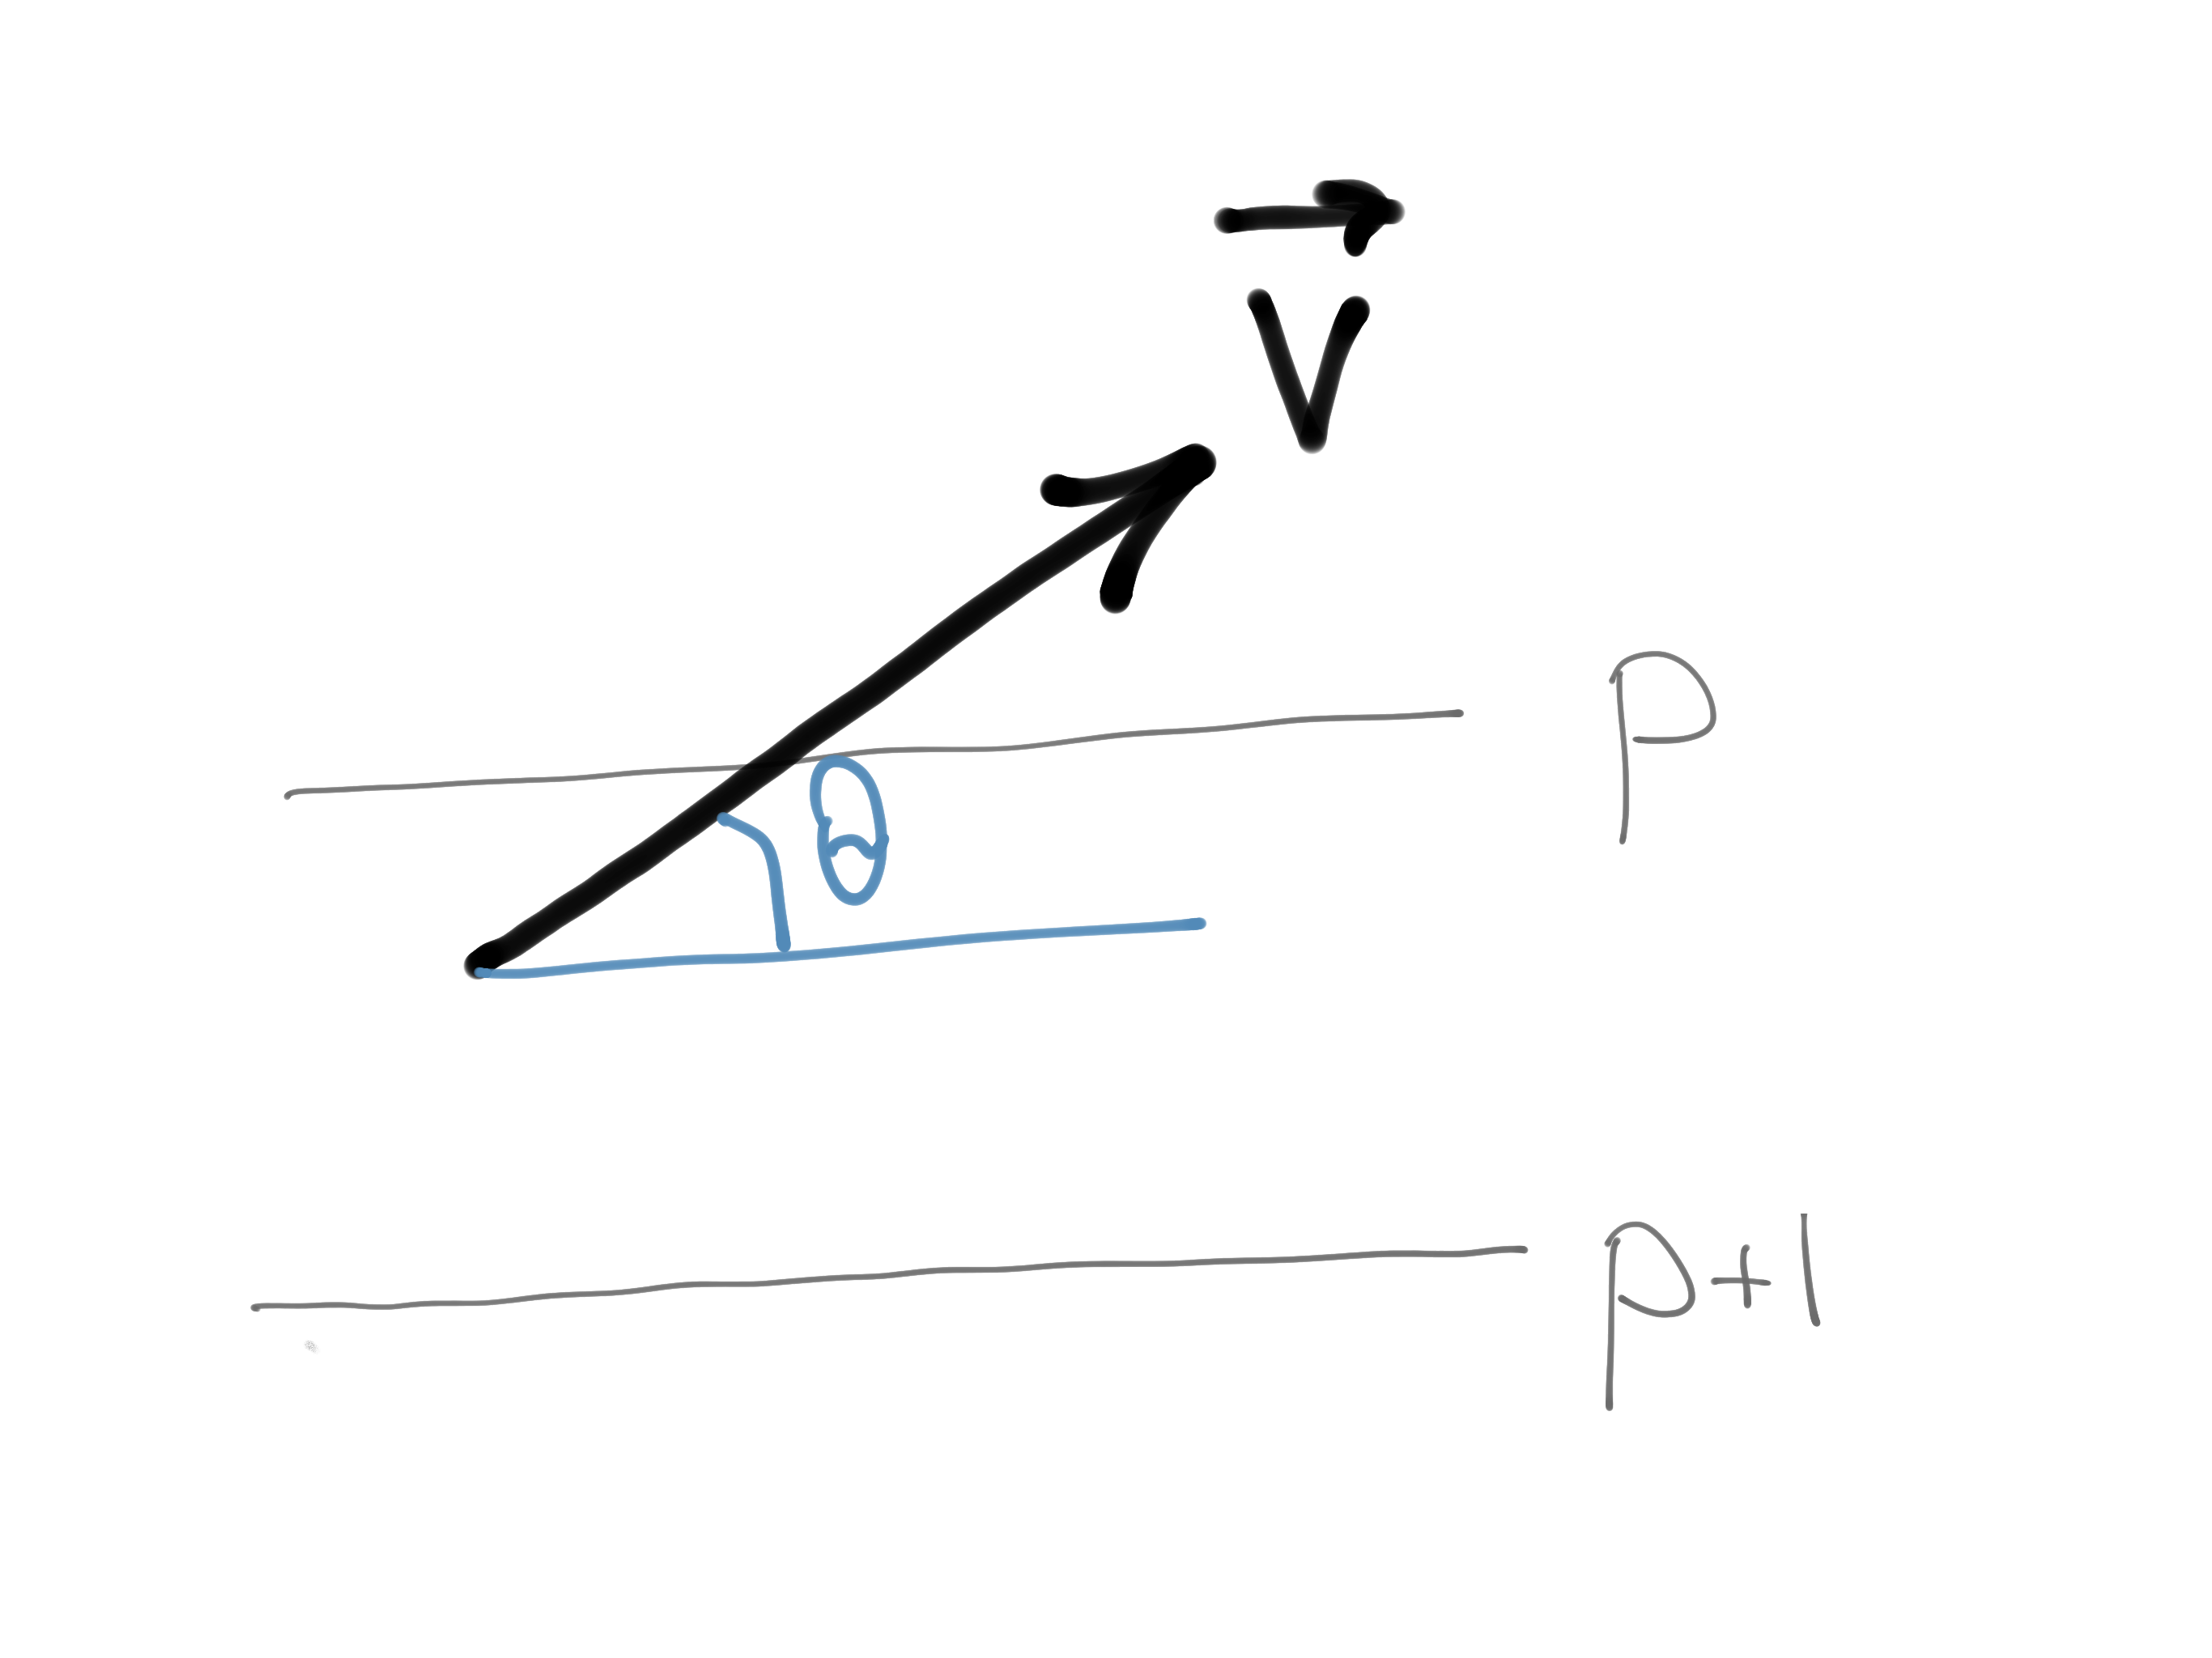
\includegraphics[width=0.5\linewidth]{pics/ch14-2_wind_turn.png}
    \caption{\label{fig:ch14-2_wind_turn} {\color{red}Схема повотора направления ветра с высотой }}
    \end{figure}
Этот угол всегда бывает острым, а его величина является функцией от высоты.

Рассмотрим теоретический вопрос об изменении скорости и направления ветра с высотой под влиянием турбулентности и отклоняющей силы вращения Земли. С движение горизонтальным и поле скорости однородным по горизонтали, будем исходить из осредненных уравнений движения атмосферы, т.е. пользоваться коэффициентом турбулентной вязкости. 

Сделаем также следующие упрощения и предположения
\begin{itemize}
    \item Движения являются стационарными и производится из линеаризация, т.е. $\td{u}{t}=\td{v}{t}=0$.
    \item Градиент давления с высотой не меняется. Поэтому, направив ось $x$ по изобаре, а ось $y$ по градиенту давления, имеем $\pd{p}{x}=0, \: \pd{p}{y}=const$.
    \item Плотность является постоянной, т.е. жидкость является несжимаемой.
    \item Коэффициент турбулентного обмена $A=\nu \rho$ является функцией постоянной
    \begin{align}
         \rho f v +A\td{^2 u}{z^2} &= 0, \label{eq:ch14-2_1} \\
        -\rho f u +A\td{^2 v}{z^2} &= \pd{p}{y}, \label{eq:ch14-2_2} 
    \end{align}
    где $f=2\omega\sin{\phi_0}$. 
\end{itemize}
Теперь сформулируем граничные условия:
\begin{itemize}
    \item[а)] у земной поверхности имеет место прилипание воздуха: 
        \begin{equation}
            \label{eq:ch14-2_3}
            u=v=0 \:\: \textrm{при} \:\: z\rightarrow0,
        \end{equation}
    \item[б)] на некоторой высоте ветер обращается в геострофический:
    \begin{equation}
            \label{eq:ch14-2_4}
            u\rightarrow u_g \:\: \textrm{при} \:\: z\rightarrow\infty.
        \end{equation}
\end{itemize}

Задачу об интегрировании системы уравнений (\ref{eq:ch14-2_1}) и (\ref{eq:ch14-2_2}) с двумя неизвестными можно свести к задаче интегрирования одного уравнения, но с комплексной неизвестной функцией
\begin{equation}
    \label{eq:ch14-2_5}
    w=u+iv
\end{equation}
Для этого умножим уравнение (\ref{eq:ch14-2_2}) на $i$ и сложим с уравнением (\ref{eq:ch14-2_1}), получим
\begin{equation}
    \label{eq:ch14-2_6}
    \rho (v-iu) + A\pd{^{2}w}{z^2} = i \pd{p}{y}.
\end{equation}
Умножив условие (\ref{eq:ch14-2_5}) на $i$ получим 
\[
iw=iu-v=-(v-u),
\]
то есть первый член в (\ref{eq:ch14-2_6}) может быть заменен из последнего выражения через $iw$ и будем иметь
\begin{equation}
    \label{eq:ch14-2_7}
    A\pd{^{2}w}{z^2} - \rho f i w = i \pd{p}{y}.
\end{equation}
Таким образом получим обыкновенное линейное уравнение второго порядка с постоянными коэффициентами, которое можно переписать с использованием соотношения для геострофического ветра следующим образом:
\[
A\pd{^{2}w}{z^2} = \phi f iw = -i f \rho u_g.
\]
Разделим все члены на $i \rho f$ и поменяем знаки членов, получим
\begin{equation}
    \label{eq:ch14-2_8}
    -\frac{1}{a^2}\pd{^{2} w}{z^2}+w = u_g, \:\: \textrm{где} \:\: a^2=\frac{\rho f}{A}.
\end{equation}

Уравнение (\ref{eq:ch14-2_8}) является неоднородным, поэтому его общий интеграл равен сумме любого частного интеграла $w_1$ этого уравнения и общего интеграла $w_2$ однородного уравнения 
\begin{equation}
    \label{eq:ch14-2_9}
    \pd{^2 w_2}{z^2} = a^2 w_2.
\end{equation}
В качестве частного интеграла уравнения (\ref{eq:ch14-2_8}), используя условие на верхней границе, можем взять 
\begin{equation}
    \label{eq:ch14-2_10}
    w_1=u_g=-\frac{1}{\rho f}\pd{p}{y}=const,
\end{equation}
т.е. скорость геострофического ветра. Общим интегралом уравнения (\ref{eq:ch14-2_9}) будет 
\begin{equation}
    \label{eq:ch14-2_11}
    w_2 = c_1 e^{az} + c_2 e^{-az},
\end{equation}
где $c_1$ и $c_2$ -- постоянные интегрирования. Складывая (\ref{eq:ch14-2_10}) и (\ref{eq:ch14-2_11}), получим общий интеграл (решение) уравнения (\ref{eq:ch14-2_8})
\begin{equation}
    \label{eq:ch14-2_12}
    w = c_1 e^{az} + c_2 e^{-az} + u_g.
\end{equation}

Произвольные постоянные интегрирования определяются из граничных условий. Так как при неограниченном возрастании $z$ скорость ветра остается ограниченной, что 
\begin{equation}
    \label{eq:ch14-2_13}
    c_1 = 0.
\end{equation}
Удовлетворяя граничному условию (\ref{eq:ch14-2_3}) при $z=0$, получим 
\begin{equation}
    \label{eq:ch14-2_14}
    c_2 = -u_g.
\end{equation}
Следовательно, окончательное решение уравнения (\ref{eq:ch14-2_8}) есть
\begin{equation}
    \label{eq:ch14-2_15}
    w = u_g (1-e^{-az}).
\end{equation}
Разделим теперь мнимую и вещественную части решения (\ref{eq:ch14-2_15}). Сначала раскроем содержание коэффициента
\[
a = \rb{ \frac{\rho f}{A} }^{1/2} = \rb{ \frac{ \rho \omega \sin{(\phi)} }{A}  }^{1/2} \cdot \rb{ 2i }^{1/2},
\]
но $(1+i)^2=1+2i-1=2i$, поэтому для $a$ можно переписать в виде
\[
a = \alpha (1+i), \:\: \textrm{где} \:\: \alpha = \rb{ \frac{\rho \omega sin{(\phi)}}{A} }^{1/2}
\]
Следовательно, (\ref{eq:ch14-2_15}) можно записать в виде, заменяя на $\alpha(1+i)$
\begin{equation}
    \label{eq:ch14-2_16}
    w = u_g \qb{ 1 - r^{-\alpha z} e^{-i \alpha z} }.
\end{equation}
Применяя формулу Эйлера
\[
e^{-i \alpha z}=\cos{(\alpha z)} - i \sin{(\alpha z)},
\]
находим 
\begin{equation}
    \label{eq:ch14-2_17}
    w = u+iv = u_g \qb{ 1-e^{-\alpha z}(\cos{(\alpha z)} - i \sin{{(\alpha z)}}) },
\end{equation}
и окончательно имеем 
\begin{equation}
  \begin{aligned}
    \label{eq:ch14-2_18}
    u &= u_g \qb{ 1 - e^{-\alpha z} \cos{(\alpha z)} }, \\
    v &= u_g e^{-\alpha z} \sin{(\alpha z)}.
  \end{aligned}
\end{equation}
Таким образом мы нашли, компоненты скорости ветра как функции скорости $C=\rb{ u^2 + v^2}^{1/2}$ и угол поворота на $\theta$:
\begin{align}
    C &= u_g \qb{ 1 - 2e^{-\alpha z} \cos{(\alpha z)} + e^{-2 \alpha z} }^{1/2}, \label{eq:ch14-2_19} \\
    \tg{\theta} = \frac{v}{u} &= \frac{ e^{-\alpha z} \sin{(\alpha z)} }{1-e^{- \alpha z}\cos{(\alpha z)}}. \label{eq:ch14-2_20}
\end{align}
Формулы (\ref{eq:ch14-2_19}) и (\ref{eq:ch14-2_20}) показывают, что по мере увеличения высоты величина скорости возрастает, а угол наклона убывает, так что ветер приближается к геострофическому. Этот процесс происходит тем быстрее, чем больше $\alpha=\rb{ \frac{ \rho \omega \sin{\phi}}{A}^{1/2} }$, т.е. чем меньше турбулентный обмен и чем больше широта $\phi$.

Из (\ref{eq:ch14-2_20}) следует, что на некоторых высотах ветер принимает направление геострофического ветра, там что $\theta=0$ при $\alpha z = \pi, 2\pi, ..., n\pi$. Наименьшая высота 
\begin{equation}
    \label{eq:ch14-2_21}
    D = \frac{\pi}{\alpha}=\pi \rb{ \frac{A}{\rho \omega \sin{\phi}} }, \:\:\: \qb{ \alpha = \frac{\rho \omega }{ A } }^{1/2} \:\: \rightarrow \:\: \qb{ \frac{  \textrm{c} }{ \textrm{м}^2 \textrm{с} } }=\frac{1}{\textrm{м}}
\end{equation}
на которой ветер принимает направление геострофического ветра, называется уровнем трения. Хотя при дальнейшем увеличении высоты ветер несколько раз отклоняется от направления геострофического ветра, но эти отклонения настолько ничтожны, что практически они не могут быть обнаружены. Это видно из таблицы \ref{tab:ch14-1}. 

\begin{table}[h]
\centering
\begin{tabular}{|c|c|c|c|c|c|c|c|c|}
\hline
\rowcolor[HTML]{EFEFEF} 
$z$ & 10 & 20 & 40 & 100 & 200 & 400 & 800 & 1200 \\
\hline
\cellcolor[HTML]{EFEFEF} $C/u_g$  & 0.075 & 0.145 & 0.286 & 0.584 & 0.893 & 1.068 & 1.005 & 0.999 \\
\cellcolor[HTML]{EFEFEF} $\theta$         & 43    & 42    & 39    & 31    & 20    & 5     & -1    & 0     \\
\hline
\end{tabular}
\caption{Изменение скорости и направления градиентного ветра с высотой (м) в планетарном пограничном слое}
\label{tab:ch14-1}
\end{table}

\begin{table}[h]
\centering
\begin{tabular}{|c|c|c|c|c|c|}
\hline
\rowcolor[HTML]{EFEFEF} 
\backslashbox{$\kappa$}{$\phi$} & $10^{\circ}$ & $30^{\circ}$ & $50^{\circ}$ & $60^{\circ}$ & $90^{\circ}$ \\
\hline
\cellcolor[HTML]{EFEFEF} 0.8  & 790      & 470      & 380      & 350      & 330      \\
\cellcolor[HTML]{EFEFEF} 4.0  & 1770     & 1040     & 840      & 790      & 740      \\
\cellcolor[HTML]{EFEFEF} 8.0  & 2500     & 1470     & 1190     & 1120     & 1040     \\
\cellcolor[HTML]{EFEFEF} 12.0 & 3060     & 1800     & 1460     & 1370     & 1280     \\
\hline
\end{tabular}
\caption{Уровень трения $D$ при разных значениях кинематического коэффициента вязкости $\kappa=\frac{A}{\rho}$ и широты местности (в метрах)}
\label{tab:ch14-2}
\end{table}
Из данных, приведенных в таблице \ref{tab:ch14-2}, видно, что с ростом турбулентного обмена уровень трения заметно повышается, а с ростом широты местности -- убывает.

Величина скорости на уровне трения получается подстановкой в (\ref{eq:ch14_19}) значения $z=D=\frac{\pi}{2}$
\begin{equation}
    \label{eq:ch14_22}
    C_D = u_g \rb{ 1 + 2e^{-\pi} + e^{-2\pi} }^{1/2} = u_g \rb{ 1 + e^{-\pi} } > u_g,
\end{equation}
больше скорости геострофического ветра.

\begin{warn}
    Пояснение (если нужно) этого вывода есть на стр. 7а  
\end{warn}

При $z=0$ формула (\ref{eq:ch14-2_20}) дает неопределенность вида $\frac{0}{0}$. Раскрывая ее по {\color{red}правилу Лопиталя (добавить в главу 1 или в Приложение )}, получим 
\begin{multline*}
  \begin{aligned}
    \lim_{z\rightarrow0}{ \tg{\theta} } &= 
    \lim_{z\rightarrow0} { \frac{ \td{}{z}\rb{ e^{-\alpha z} \sin{(\alpha z)} } }
        { \pd{}{z} \rb{ 1-e^{-\alpha z} \cos{(\alpha z)} } } } = \\
    &= \lim_{z\rightarrow0} {  
        \frac{ \cancelto{1}{-\alpha e^{-\alpha z}} \cancelto{0}{\sin{(\alpha z)}} + 
            \cancelto{1}{e^{-\alpha z}} \cancelto{1}{\cos{(\alpha z)}} \cdot \alpha }
        { \alpha \cancelto{1}{e^{-\alpha z}} \cancelto{1}{\cos{(\alpha z)}} + 
            e\cancelto{1}{^{-\alpha z}} \cancelto{0}{\sin{ (\alpha z) }} \cdot \alpha } } = 
    \frac{0+\alpha}{\alpha+0} = 1.
  \end{aligned}
\end{multline*}
Таким образом у земной поверхности угол отклонения при всех условиях равен $45^{\circ}$. 

Построив по данным таблицы \ref{tab:ch14-2} диаграмму скорости ветра как функцию от $z$, получим спираль, которая известна в геофизике под названием экмановской спирали в честь Экмана, впервые решившего вопрос об изменении направления морских течений под влиянием турбулентности и силы Кориолиса. Спираль Экмана является равноугольной логарифмической спиралью с углами в $45^{\circ}$ (см. рис. \ref{fig:ch14-2_ekman}). Она проходит из начала координат и асимптотически приближается к точке $C=u_g$.

    \begin{figure}[h]
        \centering
        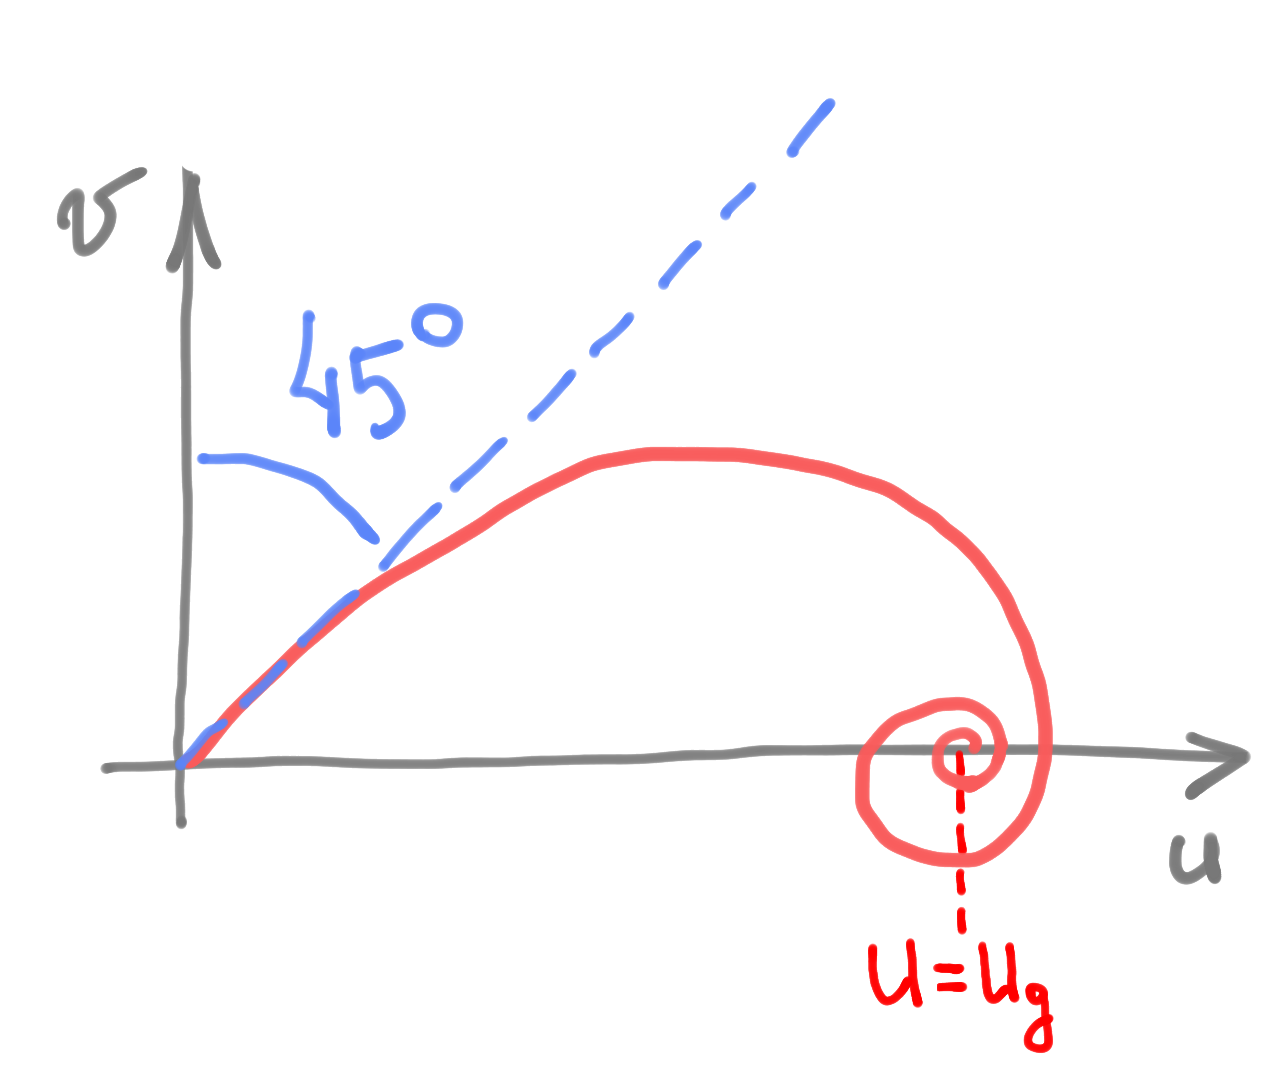
\includegraphics[width=0.5\linewidth]{pics/ch14-2_ekman.png}
    \caption{\label{fig:ch14-2_ekman} {\color{red} Спираль Экмана }}
    \end{figure}

Итак, мы установили, что в планетарном пограничном слое скорость с ветра с высотой увеличивается, поворачиваясь одновременно вправо (в северном полушарии).

Завершая этот раздел отметим дополнительно, что при выводе уравнений для составляющих скорости предполагалось, что стратификация атмосферы является нейтральной. Угол отклонения ветра от геострофического у поверхности Земли ($45^{\circ}$) нереалистично велик. Это является следствием гипотезы о постоянстве коэффициента турбулентного обмена и асимптотических граничных условий. 

\section{Профили метеорологических величин в 
нейтрально стратифицированном пограничном слое}

\section{Обобщение теории логарифмического пограничного слоя на случай стратифицированной среды}

